%%%%%%%%%%%%%%%%%%%%%%%%%%%%%%%%%%%%%%%%%
% Structured General Purpose Assignment
% LaTeX Template
%
% This template has been downloaded from:
% http://www.latextemplates.com
%
% Original author:
% Ted Pavlic (http://www.tedpavlic.com)
%
% Note:
% The \lipsum[#] commands throughout this template generate dummy text
% to fill the template out. These commands should all be removed when
% writing assignment content.
%
%%%%%%%%%%%%%%%%%%%%%%%%%%%%%%%%%%%%%%%%%

%----------------------------------------------------------------------------------------
%	PACKAGES AND OTHER DOCUMENT CONFIGURATIONS
%----------------------------------------------------------------------------------------

\documentclass{article}
\usepackage[utf8]{inputenc}
\usepackage[T1]{fontenc}
\usepackage{lmodern} % load a font with all the characters
\usepackage[]{algorithm2e}
\usepackage{minted}

\usepackage{fancyhdr} % Required for custom headers
\usepackage{lastpage} % Required to determine the last page for the footer
\usepackage{extramarks} % Required for headers and footers
\usepackage{graphicx} % Required to insert images
\usepackage{lipsum} % Used for inserting dummy 'Lorem ipsum' text into the template
\usepackage{underscore}
\usepackage{graphicx}

% Margins
\topmargin=-0.45in
\evensidemargin=0in
\oddsidemargin=0in
\textwidth=6.5in
\textheight=9.0in
\headsep=0.25in

\linespread{1.1} % Line spacing

% Set up the header and footer
\pagestyle{fancy}
\lhead{\hmwkAuthorName} % Top left header
\chead{\hmwkTitle} % Top center header
\rhead{\firstxmark} % Top right header
\lfoot{\lastxmark} % Bottom left footer
\cfoot{} % Bottom center footer
\rfoot{Page\ \thepage\ of\ \pageref{LastPage}} % Bottom right footer
\renewcommand\headrulewidth{0.4pt} % Size of the header rule
\renewcommand\footrulewidth{0.4pt} % Size of the footer rule

\setlength\parindent{0pt} % Removes all indentation from paragraphs

%----------------------------------------------------------------------------------------
%	NAME AND CLASS SECTION
%----------------------------------------------------------------------------------------

\newcommand{\hmwkTitle}{Searching the space of word temporal profiles on Le Temps Newspaper } % Assignment title
\newcommand{\hmwkDueDate}{Monday,\ May 18,\ 2015} % Due date
\newcommand{\hmwkClassTime}{} % Class/lecture time
\newcommand{\hmwkClassInstructor}{} % Teacher/lecturer
\newcommand{\hmwkAuthorName}{} % Your name

%----------------------------------------------------------------------------------------
%	TITLE PAGE
%----------------------------------------------------------------------------------------

\title{
\vspace{2in}
\textmd{\textbf{\hmwkTitle}}\\
\normalsize\vspace{0.1in}\small{Due\ on\ \hmwkDueDate}\\
\vspace{3in}
}

\author{Sidney Bovet \and Valentin Rutz \and Zhivka Gucevska  \and Mathieu Monney\and Florian Junker\and John Gaspoz\and Joanna Salathé\and Ana Manasovska\and Fabien Jolidon}
\date{\today} % Insert date here if you want it to appear below your name

%----------------------------------------------------------------------------------------

\begin{document}

\maketitle

%----------------------------------------------------------------------------------------
%	TABLE OF CONTENTS
%----------------------------------------------------------------------------------------

%\setcounter{tocdepth}{1} % Uncomment this line if you don't want subsections listed in the ToC

\newpage
\tableofcontents
\newpage


\section{Motivation}
Studies based on the visualization and analyses of temporal profile of word using a so-called “n-gram” approach have been popular in the last years. However, most of the studies so far discuss the case of remarkable words, most of the time found thanks to the researcher’s intuitions for finding “Interesting” curves using the n-gram viewer.\\

The motivation of this project is to invert the problem and to propose a simple tool for researchers to automatically explore the space of temporal curves in search for words. As researchers often analyse how words appear and relate to historical events, our goal was to provide researchers a way to extract words having the same temporal profile. These results would help the researchers to analyze the use of a given word and the events that they relate to. \\

In order to classify the temporal profiles various metric were implemented providing the user different ways to retrieve interesting information. \\

In section 2, we will explain how the data generation was made. From parsing the OCR'd articles to a cleaned and formatted data. In Section 3 we detail how the application is structured and its general pipeline. Section 4 describes in details the metrics implemented as well as their strengths and weaknesses. Section 5 and 6 describe how we proceeded to optimize the metric's parameter and how the metrics perform against some test cases. Finally, section 7 provides hints about future works that could fit this project.\\

Our analysis is based on Le Temps Newspaper Corpus which is a database of 4 million articles covering a period of 200 years and composed of digitized facsimiles of "Le Journal de Genève" and "La Gazette de Lausanne" wherein each article has been OCR'd.



\section{Data Generation}
Data generation is a critical component as messy data will impact the accuracy of the metrics and the pertinence of its outputs. Hence, great care was taken in the data generation phase in order to make the data as useful as possible for the application. With the use of various statistics we were able to filter many garbage data.

\subsection{Parsing}
This part is responsible for taking the raw input (OCR’d articles) and output only the interesting information. Its output is a set of files written in UTF-8. Each file contains a list of words, possibly with repetition, that occur the same year and separated by a space. The first word of each file is the year on which all following words occur. Therefor a typical output file is [year word1 word2 word3 ...]\\

The first thing we do is to get rid of all meta data except the year of release. We are left with a set of article contents that we process as if there are a list of words separated by space. Of course, this doesn't correspond to reality since some word could have a "." at their end or others could have a determiner such as "l'" at their beginning. This is why for we try to clean the article the more we can as early as we can. To get rid of all special characters we use a regex "\textbackslash p\{L\}" that return all letters including letters with accent. Then we take care of some special case such as determiner with an apostrophe or words with hyphen. Finally, we write the result in a file with the corresponding year. The output of parsing corresponds to the input of 1gram Generation.

\subsection{1gram Generation}
To ease the development of the metrics we defined that for each word we would have a list of 159 Integer entries containing the number of occurrences for this word for each year in the range of our database ( from year 1840 to 1998).\\

In order to compute this, two map reduce functions were created. The parsing phase had given a list of files, one file for a year, containing every word used in that year. The first mapreduce would process each of these files and output, in a file, each word associated with the year and occurrences for this year : [year\_word occurrences].\\

The second mapreduce would take, as input, the output of the first one and generate the final format [word occurence\_year1, occurence\_year2, ...]. If no occurrence of a word was found for a year a 0 value would be assigned to this specific year.

\subsection{1gram Cleaning}

\section{Architecture}
This section details the whole application's architecture. It describes the whole operation's pipeline and the main components of the Backend and the Frontend.
\subsection{Backend Architecture}

\subsubsection{General overview}
Our backend architecture is composed of four main types of elements namely: SparkCommander, Launcher, similarity techniques and utils functions.\\

Before describing those elements separately in greater details, you can find hereafter the link between them in this “pipeline-fashion” picture.

\begin{figure}[ht!]
\centering
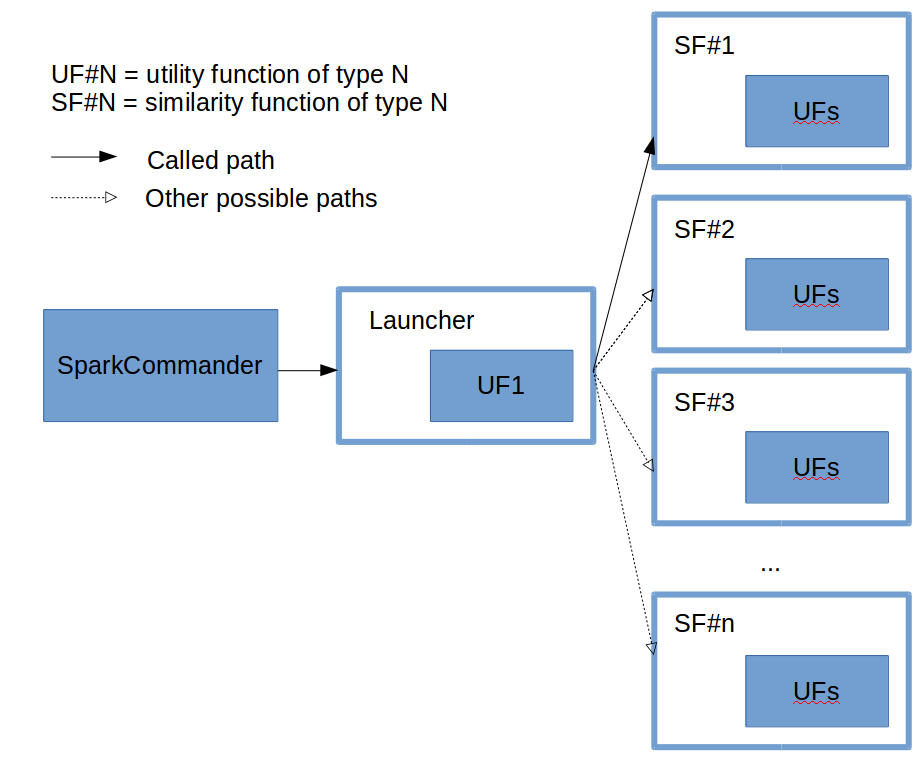
\includegraphics[width=90mm]{reportBackendGeneralPipeline.png}
\caption{Backend General Pipeline \label{overflow}}
\end{figure}



\subsubsection{SparkCommander}
SparkCommander is the link between the frontend and the backend. It is the main class of our backend and its purpose is to choose the similarity technique (see section \ref{Similarity techniques} and the mode (find similar words for a specific word or for a list of words) from the parameters it received from the front end. It then decides from those parameters how to call the Launcher.

\subsubsection{Launcher}
Launcher is the backbone of the similarity function process. Its purpose consists of three steps: formatting, applying a similarity techniques and finally preparing the display for the front end.

\subsubsection{Similarity techniques}
Each technique must follow the same signature i.e \texttt{(data: RDD[(String, Array[Double])], testedWord: (String, Array[Double]), parameters: List[Double]): RDD[(String)]]} 
 and apply this pipeline:\\

\begin{figure}[ht!]
\centering
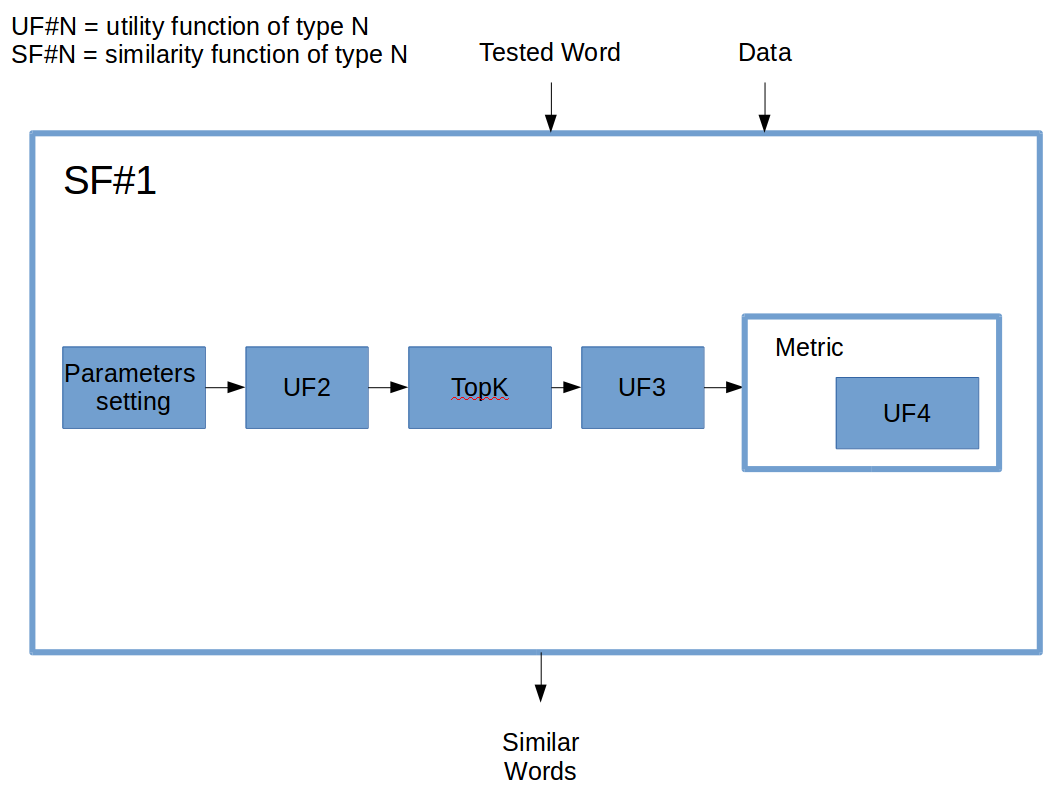
\includegraphics[width=90mm]{reportBackendSFPipeline.png}
\caption{Backend SF Pipeline \label{overflow}}
\end{figure}



More precisely each technique will first assign parameters it received from the Launcher to use them, then it will call topK a special utils function that will output the k most similar words (see section \ref{Utils functions} for more details), after that it can apply other utils functions and finally it will call a specific metric (i.e. a function that gives a similarity score for ranking the words contained in the data it received, for more information see section \ref{Metrics}).

\subsubsection{Utils functions}
The utils functions are, as the name suggests, function that are useful in different places.\\

Roughly speaking, there exists 5 utils classes:


\begin{enumerate}
\item Used by the Launcher (for formatting and displaying)
\item Used to apply sub techniques before a similarity technique
\item Used to transform the data (for scaling or smoothing)
\item Used for computation purpose (e.g. variance, finding min and max and so on)
\item Used to retrieve the topK
\end{enumerate}


As seen on the precedent pictures those functions are used in different places (UF1 correspond to [1], UF2 to [2], UF3 to [3] and finally UF4 mainly to [4] but can also be found in other places from time to time.\\

Concerning  [5] it was explicitly written under TopK label on the precedent figure and is necessarily implemented by each similarity function. It’s purpose is, given the similarity score computed by the metric (see section \ref{Metrics}), to rank the words and output the k most similar one.




\subsection{Frontend Architecture}

We decided to use Play with Scala as a framework to be able to use Spark in the backend as well as a well designed framework for intercepting HTTP requests.
It allowed us to begin quickly with the implementation of the metrics. \\

So at this point, we had a simple web interface where users would be able to enter words, use the REST API of the Play framework to send a HTTP POST with the words he/she wants to search.
Then Play would send it to the right controller which would run the selected technique with the Spark API for Scala. We would take each word with its occurrences and give it to the technique with the rest of the data. \\

Then 3 options could happen: either the word was not in the data, which would mean that we could not have any results, or the word was in the data but there was no similar words for the given parameters or, last option, we get back from the technique a set of words that were deemed similar with respect to the technique and the parameters.
For the first two outcomes, we would only send back the information that it was not in the data or had no similar words but if there was results, then we would send all of those words back to the browser in a JSON and display  them. \\

At that moment, we were doing all local testing since it was early in the project and the parsing/cleaning/generation of the data was not yet complete. Then we were told that it would not be possible to put the Play project directly running on the cluster so we had to think of some other way to interact with the cluster. \\

One way we had found, was simple and was to connect directly with the URL to Spark on the cluster. This can be done using the function SparkConf.setMaster(master_URL) and put the master URL to icdataporal2:<some_port>/<spark_URL> but since the cluster was using YARN as the resource manager, it was not possible to use this way to keep the structure as was. One possibility that Immanuel pointed out was to separate the Spark part of the project from the server side talking to the browser. We would put all techniques in a jar on the cluster and launch Spark job using SSH from Play. \\

This was the simplest and quickest solution to implement and is the final architecture we have. 
The simple interface allows the user to put at most 4 words (more would just overload the interface once the results arrive), choose a technique, and put all parameters for this technique to be able to run. \\

Then when the user clicks on the button, the interface will gather all of these inputs, put them in a JSON as: 
\begin{listing}
\begin{minted}[frame=single,
               framesep=3mm,
               linenos=true,
               xleftmargin=21pt,
               tabsize=4]{js}
{
	words: [word1, ...],
	technique: name,
	parameters: [parameter1, ...]
}
\end{minted}
\caption{JSON example} 
\label{json-example}
\end{listing}



The parameters are optional depending on how the person who implemented the technique wanted to do it.

One problem with this part is that nowadays, browser do not like make HTTP requests that are not GET.
So each time a browser does an HTTP POST, DELETE, PUT, or else, it will make a preflight request OPTIONS to the server and if not all the responses from the server have the header "Access-Control-Allow-Origin" to "*", it will be an error for the browser.
Thankfully, Play can intercept all response from the controllers and add that header using filter (see app/filters/CORSFilter.scala for the intercepter and app/Global.scala for its use).
When the request with the JSON from the browser arrives to the controllers, it is parsed from JSON to a JsValue (Play JSON API) and then we extract the words, technique name and parameters.
We have now everything we need to launch the Spark job on the cluster.

First, we used the scala-ssh library (https://github.com/sirthias/scala-ssh) to make the SSH connection from the server to the cluster.
For that every team member has a local file ~/.scala-ssh/icdataportal2 where there are all details such as username, key file, etc... to create the SSH connection.
Then, we saw that Spark could be slow for a demo since it has to communicate to its nodes so as Immanuel proposed we decided to do a bit of preprocessing of the data but we did not want to loose all the work we did at the moment so instead of trying to preprocess everything, we implemented a "dead cache", i.e. when we have a request from the browser, we first test using the command "hadoop fs -test -d " + hdfsResDir + "/results" where hdfsResDir is the path where the result is in the cache. 
If this directory exists, then instead of launching a Spark job for something that has already been computed, we simply use "hadoop fs -getmerge " + hdfsResDir + "/results" to merge all results from Spark to the local accoount on the cluster of the user, then download it using SCP to the Play server.
The server will then parse the result which has the form:
word1 -> match1 match2 match3 ...
word2 -> NOTINDATA
word3 -> NOSIMILARWORDS
We use scala.utils.parsing.combinators to create this parser (see it in app/utils/ResultParser.scala) and then use the Play JSON API to transform it into JSON and send it to the browser that will be able to easily display it.
If the search has never been attempted, then we launch the spark job using the command: "spark-submit --class SparkCommander --master yarn-cluster <other spark options> SparkCommander-assembly-1.0.jar -w word1, ... -t technique_name -p param1, ...".
Then we follow the same protocol as if the search had already been done.

For testing purposes, we needed aa way to plot the temporal profiles of words and similar words.
We used the dimple.js library based on d3.js (http://dimplejs.org/) to display graphically those words.
It takes a csv file and display the data given as Word,Year,Occurrences.
We also created another page only to display the words the user wants.
It is not going to search for similar words but just query the data via Spark to get all the occurrences of a word (or a series of words), write them in the csv file, then the server downloads it and sends it back to the client as before (see it in src/main/scala/DisplayCommander.scala)

The part where we search similar words submits the SparkCommander job on Spark, it uses the scopt library (https://github.com/scopt/scopt) to extract the words, technique name and parameters.
then we use the technique name to retrieve the similarity function to be applied and use the function runList(words, input, baseprofile, output, parameters, similarityTechnique, sparkcontext, range).
This will apply the similarity technique for each word with the parameters, the range needed, etc...
Then we save in a text file the results for each words and the data to graph as well.

Problems encountered and solutions:
	- No possibility of running on the cluster -> use SSH and SCP to communicate with SparkCommander and DisplayCommander
	- HTTP requests other than GET end up in an error at the browser -> use CORS in Play to be able to communicate
	- Time to process a request can be long depending on the size of the result set -> implement a dead cache that will speed up the next queries
	- No hadoop command on the default shell on the cluster -> put them in the .cshrc or use "bash -c \"source .bashrc; <cmd>\"" 
	- Please everyone -> work hard!

\begin{figure}[ht!]
\centering
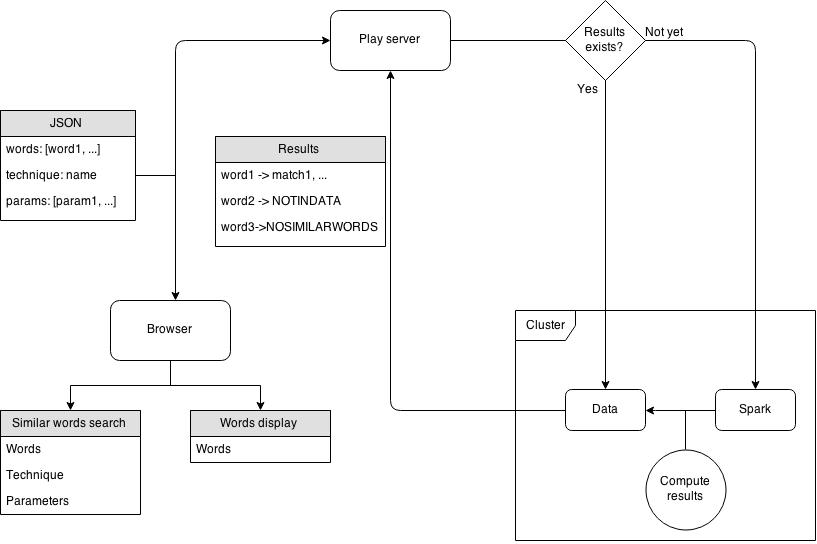
\includegraphics[width=90mm]{Flowchart.jpg}
\caption{Flow Chart \label{overflow}}
\end{figure}


\section{Metrics}

The metrics are used, as briefly explained in the previous section (\ref{Backend Architecture}, by the topK utils function to output a ranking of similar words. Therefore the goal of each metric is to give a score between two words in relation with their similarity degree. For that purpose each metric must follow this signature: \texttt{word1Freq: (Array[Double]), word2Freq: (Array[Double]), parameters: List[Double] = List()): Double}//

Thereafter we will present you each metric separately. We will first present you with which similarity techniques they are used, then we will talk about the algorithm they use and finally we will present what are their good points and bad points.


\subsubsection{Curve Comparison Difference}

This metric is used when calling NaiveComparison similarity technique. The main idea of this metric is to compute the difference between each point of the two arrays. The output for the scoring is the average of those differences. That is, the greater the difference, the less similar two arrays are. \\

The input of this technique is a double value: acceptedDifference. This input is used to penalize too extreme value. For that purpose we will filter the elements at index i of the arrays if the difference between them is greater than the acceptedDifference. Therefore the average sum will become greater since the length of the array of differences are smaller.\\

More formally the algorithm is: “TODO joli en Latex”\\

The good point of this metric, which can also be seen as a bad point is that it is very strict. More precisely, with this metric, we are always comparing the same year and don’t accept that the shape could be a bit shift one year later but still similar. (see \ref{Dynamic Time Warping} for this behaviour). Though, this technique will clearly fail in one specific case, namely the curve where the words appeared only at the very end of our years range. Why that? In fact before this apparition the frequency of the word will be 0 and will have a lot of “common match” with all the other words that appeared also only at the end of our year range. The main problem is that in this case roughly 80% of the similarity will be computed because both curve are flat at the beginning, which is not a good similarity indicator.


\subsubsection{Curve Comparison Division}

\subsubsection{Peak Detection}

This metric is used when calling $PeakComparison$ similarity technique. \\
\\
We have decided to implement a metric that will compare curves by detecting the peaks in each curves based on our analysis on the provided data. We have noticed that some words that are related to a specific event, are more mentioned in the years of the event. A nice example for that is the word $"guerre"$, which has big peaks in 1940 and 1945 or the word $"olympique"$, which has peaks every 4 years.\\

The main idea behind this metric is, given two words, find the peaks for each of them and count the years in which peaks were detected in both. After that look at the percentage of different peaks from all the peaks for each of them, and output the larger values. This means, the smaller the result of this metric is, less there were different peaks in the temporal profiles, hence more similar the two profiles are.\\
\\
The algorithms for detecting peaks use $2$ $parameters$:
\begin{itemize}
\item $windowSize$ This parameter is used for finding the widest ascending(or descending) window and his purpose is to allow variations in the latter. To find the widest ascending (or descending window), we use a moving average, and this window decides how many points are considered in the moving average. This window also defines the deviation on the $x-axis$. That is, if the moving average considers very few, say two values, then the peaks will be narrow, and no shift on the axis should be allowed. However, if this window is large, this means that some variances were allowed, and even though the peaks of two curves overlap, they are not detected in the same year, so some shift in the years can be tolerated.
\item $ratio$ This parameter is used to define the peak: that is, if we have the lowest point of the peak, and the highest, and look at their ratio, from what point do we consider that the growth was drastic enough to be considered as a peak.
\end{itemize}

%\begin{algorithm}
%\caption{Peak detection algorithm}
%\label{PeakDetectionAlgorithm}
%\begin{algorithmic}[H]
%\Procedure{Detect\textendash Peaks}{frequencies, windowSize, ratio}
%\While{$i$ < $N$ }
%\State let $f_1=findAscendingWindow(frequencies, i, windowSize)$
%\State let $j_1$ be the index of the maximum in $f_1$
%\State let $j_2$ be the index of the minimum in $f_1$
%\State \textbf{if} ($j_1$ = $j_2$) $i$++; \textbf{continue}
%\State let $f_2 = findDescendingWindow(frequencies, j_1, windowSize)$
%\State let $j_3$ be the index of the minimum in $f_2$
%\State \textbf{if} ($j_1$ = $j_3$) $i$++; \textbf{continue}
%\State \textbf{if} (value of $j_1$ < ratio $\times$ \text{ $min$(value of $j_2$, $j_3$) $i$++; \textbf{continue}}
%\State add year corresponding to $j_2$ to $peaks$
%\EndWhile
%\State \Return $peaks$
%\EndProcedure
%\end{algorithmic}
%\end{algorithm}

The $findAscendingWindow$ and $findDescendingWindow$ are quite similar, here is example for the first one:



\subsubsection{Dynamic Time Warping}

\section{Data Tuning}

For the data tuning we use test cases, each of which consists of 1 word and 2 lists of words; the first list contains words that should match the given word, and the second list contains words that shouldn’t match the given word.\\

The data tuning takes each metric and each test case and tries to find the best parameters by trying several values in a given range. For every set of parameter it will compute a “grade” based on how many words from the test case were in the set of words returned by the metric, and it will keep the parameters that gives the best “grade”. The grade is computed by taking the average between the ratio of words from the “should match” test case that are in the result and the ratio of words from the “should not match” test case that are not in the result.

\section{Experimental results}
\subsection{Metric Benchmark}

\section{Conclusion and Future work}

As observed in the previous section, with the use of this application we were able to retrieve interesting information. For example, by testing the word "guerre" we detected various semantically similar words as output. And by looking at their temporal profiles we can analyse when these words were mostly used and observe that their pic of occurrences would match the historic event of the first and second war. \\

This a simple test-case but it shows that, giving a word, the user can retrieve useful information. Hence researcher can use the application to verify its intuition but also to discover retrieve unexpected information related to a word. Of course not all words would give such interesting results and, as we saw previously, not every metric performs well for any words.


 \end{document}


\end{document}



